\documentclass{beamer}

\usepackage[ngerman]{babel}
\usepackage[utf8]{inputenc}
\usepackage[T1]{fontenc}
\usepackage{lmodern}

\usepackage[german,linesnumbered,algoruled,longend,vlined]{algorithm2e}
\DontPrintSemicolon
\SetArgSty{}
\SetKw{KwOr}{or}
\SetKw{KwAnd}{and}
\SetKw{KwNot}{not}
\setlength{\algomargin}{3ex}

\usepackage[fixlanguage]{babelbib}
\setbibliographyfont{title}{}
\setbibliographyfont{jtitle}{}
\setbibliographyfont{btitle}{\emph}
\setbibliographyfont{stitle}{\emph}
\setbibliographyfont{journal}{\emph}

\usepackage{amsmath}
\usepackage{amsfonts}
\usepackage{amssymb}
\usepackage{amsthm}

\usepackage{graphicx}
\usepackage{enumerate}
\usepackage{textcomp}
\usepackage{epstopdf}

\graphicspath{{graphics/}}

% Eigene Commands:
\newcommand{\Epsilon}{\mathcal{E}}
\newcommand{\N}{\mathbb{N}}

\hyphenation{Teil-as-pekt Teil-as-pek-te}

\begin{document}



\subject{Algorithmen für geographische Informationssysteme}
\title{Projekt Viewshed Analysis}
\author{Christina Hempfling, Jona Kalkus, Moritz Beck, Bernhard Häussner}
\date{Projekt-Präsentation am 15. Juni 2015}
\institute{Julius-Maximilians-Universität Würzburg\\
Institut für Informatik\\
Lehrstuhl für Informatik I\\
Effiziente Algorithmen und wissensbasierte Systeme\\[\baselineskip]
Betreuer:\\ 
Prof.\ Dr.\ Alexander Wolff\\
Dr.\ Thomas van Dijk\\
Benedikt Budig, M.Sc.}
\maketitle


\section{Einleitung}

\begin{frame}
  \frametitle{Was ist Viewshed Analysis?}
  \begin{itemize}[<+->]
    \item Eingabe: Digitales Höhenmodell (DEM),
    \item Standpunkt und Höhe im DEM
    \item Ausgabe: Sichtbarer Bereich vom Standpunkt aus
    \item Anwendung: Aufstellen von Sendemasten, finden versteckter oder landschaftlich attraktiver Routen
  \end{itemize}
\end{frame}

\begin{frame}
  \frametitle{Ein Beispiel}
  \begin{figure}[h]
    \centering
    \fbox{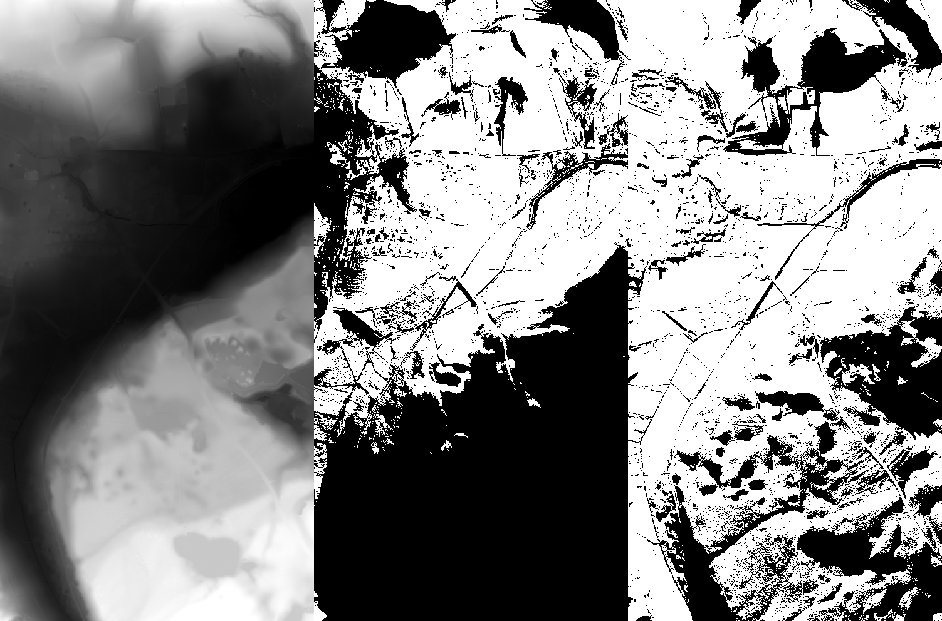
\includegraphics[height=5cm]{example}}
    \caption{Ein DEM (links) und zwei Viewsheds}
    \label{fig:example}
  \end{figure}
\end{frame}

\section{Algorithmen}

\begin{frame}
  \frametitle{Der Brute-Force-Algorithmus}
  \begin{itemize}[<+->]
    \item Für jeden Punkt des DEM
    \item Finde alle Punkte zwischen diesem und dem Standpunkt
    \item Prüfe für diese Punkte, ob sie größere Steigung haben
    \item Hat keiner größere Steigung, ist der Punkt sichtbar, sonst nicht
    \item Laufzeit $O(n^3)$ ($n$ Breite des DEM, gewöhnlich rund 1k)
  \end{itemize}
\end{frame}


\begin{frame}
  \frametitle{Verbesserung: Sweepline (van Krefeld~\cite{van1996variations})}
  \begin{itemize}[<+->]
    \item 
    \item 
    \item 
    \item 
  \end{itemize}
\end{frame}


\begin{frame}
  \frametitle{Verbesserungsidee: Quad Trees}
  \begin{itemize}[<+->]
    \item 
    \item 
    \item 
    \item 
  \end{itemize}
\end{frame}

\section{Probleme}

\begin{frame}
  \frametitle{Probleme: Linie berührt Pixel}
  \begin{itemize}[<+->]
    \item 
    \item 
    \item 
    \item 
  \end{itemize}
\end{frame}

\begin{frame}
  \frametitle{Probleme: Interpolation des DEM~\cite{fisher1993algorithm}}
  \begin{itemize}[<+->]
    \item 
    \item 
    \item 
    \item 
  \end{itemize}
\end{frame}

\begin{frame}
  \frametitle{Probleme: Artefakte an Winkelhalbierenden}
  \begin{itemize}[<+->]
    \item 
    \item 
    \item 
    \item 
  \end{itemize}
\end{frame}

\begin{frame}%[shrink=30]
  \frametitle{Literatur}
  \bibliographystyle{mybabalpha-fl}
  \small\bibliography{mybib}
\end{frame}




\end{document}